\section{Front Trees}
\label{section:front-trees}
\par
To illustrate the different types of front trees, and their
transformations we do for the sake of efficiency,
we will use an an example the matrix R2D100, a matrix generated by
first randomly triangulating the unit square with 100 grid points.
The resulting matrix has 100 rows and columns.
We ordered the matrix using a generalized nested dissection
algorithm from the {\bf SPOOLES} library. 
On the left in Figure~\ref{fig:R2D100} is the triangulation.
On the right we have labeled the grid points with their place in
the nested dissection ordering.
Note that vertices 90 through 99 form a separator of the graph.
Vertices 0 through 47 are found on the right of the separator, 
vertices 48 through 89 are found on the left
\par
\begin{figure}[htbp]
\caption{R2D100: randomly triangulated, 100 grid points}
\label{fig:R2D100}
\begin{center}
\mbox{
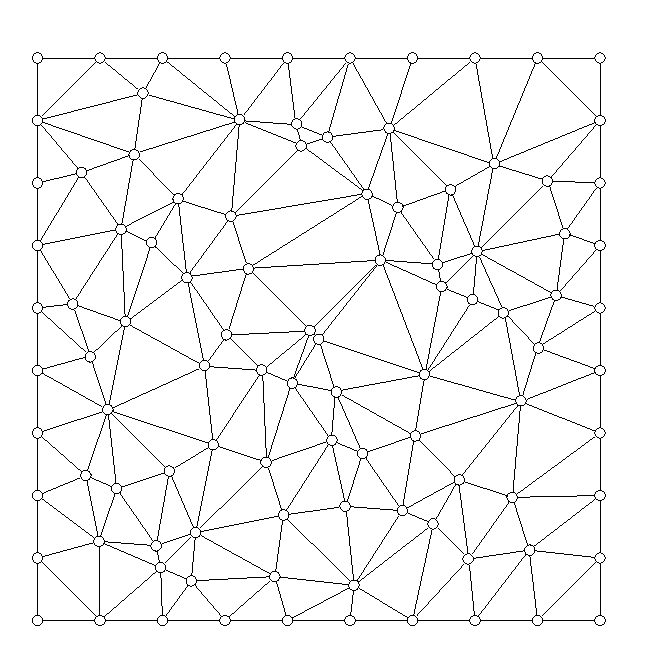
\psfig{file=R2D100.eps,width=3.0in,height=3.00in}
}
\mbox{
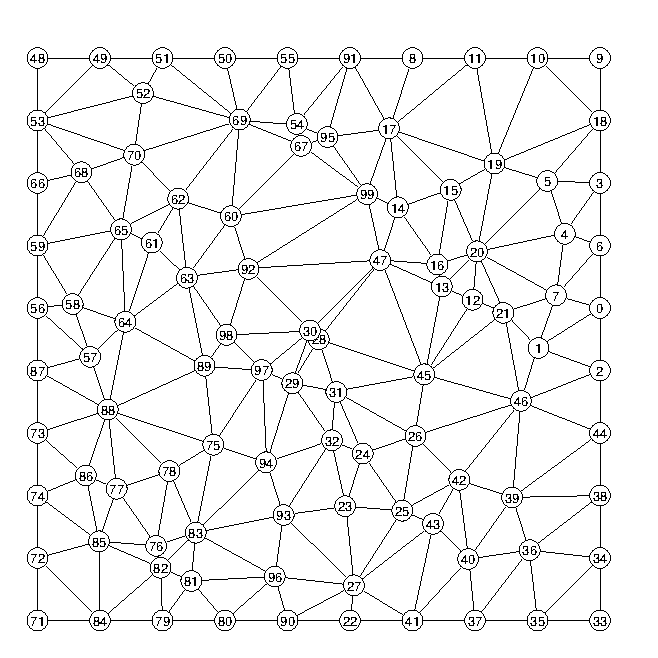
\psfig{file=R2D100perm.eps,width=3.0in,height=3.00in}
}
\end{center}
\end{figure}
\par
\subsection{Vertex elimination trees}
\label{subsection:vtx-elim}
\par
Recall that the four ordering methods from
Section~\ref{section:ordering} return an {\tt ETree} object.
% In addition to the tree structure, an {\tt  ETree} object contains 
% other information: the number of internal and external rows 
% and columns to a
% front, and a map from each row and column to the front it belongs in.
There is another way to construct a tree using the {\tt Graph} object
and the permutation vectors.
The following code fragment shows how to do this.
\begin{verbatim}
ETree   *vetree ;
int     *newToOld, *oldToNew ;
Graph   *graph ;

vetree = ETree_new() ;
ETree_initFromGraphWithPerms(vetree, graph, newToOld, oldToNew) ;
\end{verbatim}
The {\tt vetree} object in the code fragment above is a
{\it vertex elimination tree} 
\cite{liu90-etree}, \cite{sch82-etree},
where each front contains one vertex.
\par
Figure~\ref{fig:R2D100-tree-vtx} contains the vertex elimination tree 
for this ordering.
The vertex elimination tree is
a representation of the partial order by which 
the vertices in the graph may be eliminated.\footnote{
Vertex $j$ is the parent of $i$ if $j$ is the first vertex greater
than $i$ such that $L_{j,i} \ne 0$.
}
The dependencies of the rows and columns form a tree structure.  
The leaves of the tree (our trees hang 
upside down with the leaves at the bottom and the root at the top)
represent vertices which can be eliminated first.  
The parents of those leaf nodes can be eliminated next, 
and so on, until finally the vertices represented 
by the root of the tree will be eliminated last.
\par
\begin{figure}[htbp]
\caption{Vertex elimination tree for R2D100, 100 rows and columns}
\label{fig:R2D100-tree-vtx}
\begin{center}
\mbox{
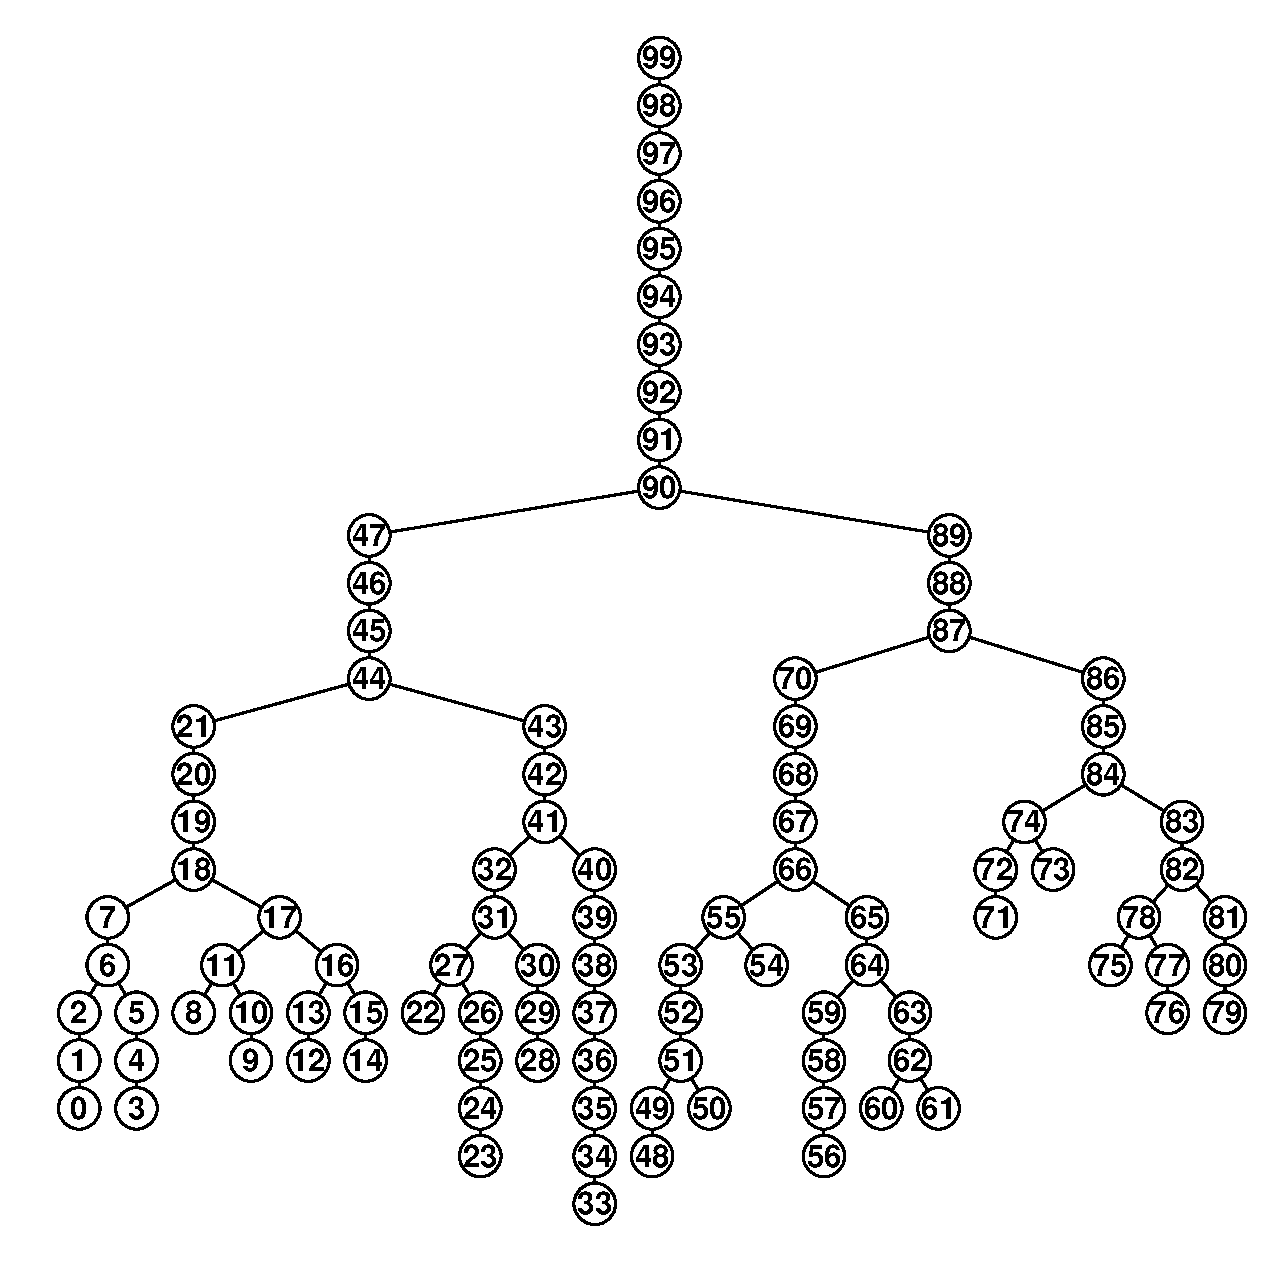
\psfig{file=vtree.eps,width=5.0in,height=5.00in}
}
\end{center}
\end{figure}
\par
The elimination tree illustrates the dependence of the vertices.
The basic  rule is that a vertex {\it depends} only on its descendents
and will {\it affect} only its ancestors.
It should be clear that the tree allows us to identify independent,
parallel computation.
For example, the computation of the factor entries in the 
subtree rooted at vertex 47 is completely independent of the
subtree rooted at vertex 89, so we could identify one process to
compute the left subtree and another to compute the right subtree.
\par
\subsection{Fundamental supernode trees}
\label{subsection:fs-tree}
\par
While the vertex elimination tree is useful to communicate the data
dependencies, it is not a good granularity on which to
base a factorization or solve, in serial or in parallel.
It is important to group vertices together in some meaningful way
to create larger data structures that will be more efficient with
respect to storage and computation.
% The first step in this direction is to group together vertices
% that form a chain with no branches in the tree.
Any grouping of vertices imposes a block structure on the matrix.
The {\it fundamental supernode tree} 
\cite{ash89-relaxed}
has these property:
any node in the tree is 
\begin{itemize}
\item either a leaf,
\item or has two or more children,
\item or its nonzero structure 
      is not contained in that of its one child.
\end{itemize}
The top tree in Figure~\ref{fig:fs-trees}
shows the vertex elimination tree with the ``front'' number of each
vertex superimposed on the vertex.
The bottom tree is the fundamental supernode tree.
Figure~\ref{fig:R2D100-fs-mtx} shows the block partition superimposed on
the structure of the factor $L$.
Note this one important property: 
within any block column and below the diagonal block,
a row is either zero or dense.
\par
\begin{figure}[htbp]
\caption{Top: vertex elimination tree with the vertices mapped to
the fundamental supernode that contains them. 
Bottom: fundamental supernode tree.}
\label{fig:fs-trees}
\begin{center}
\mbox{
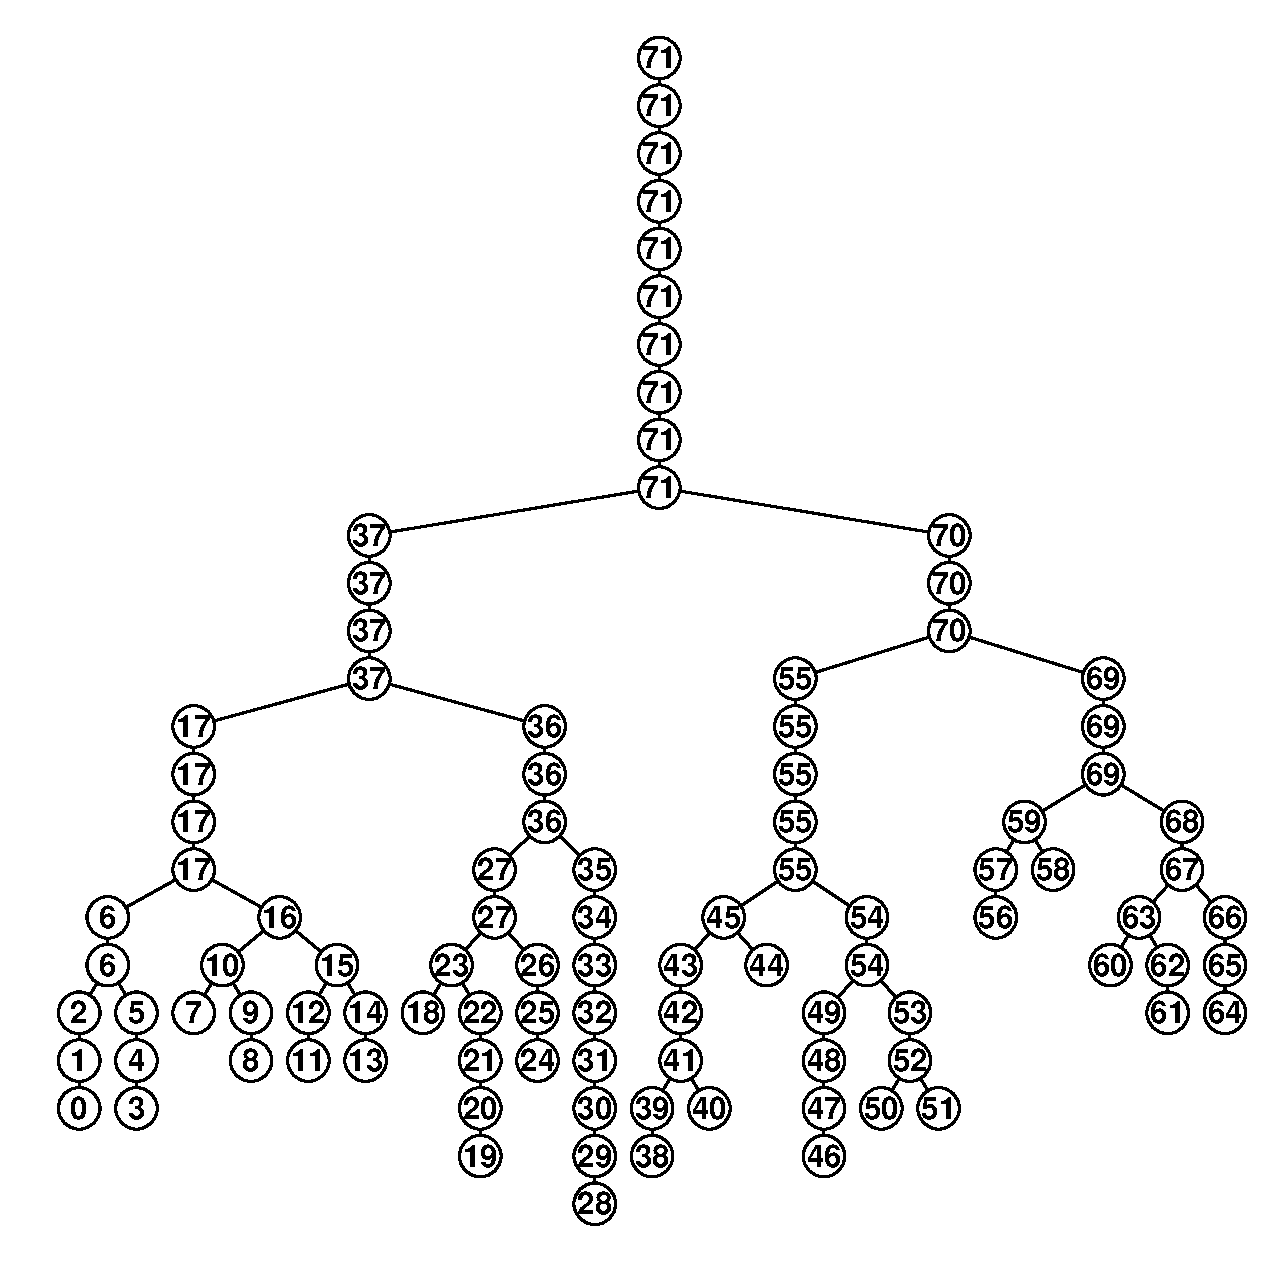
\psfig{file=fsvtree.eps,width=5.0in,height=5.00in}
}
\par
\mbox{
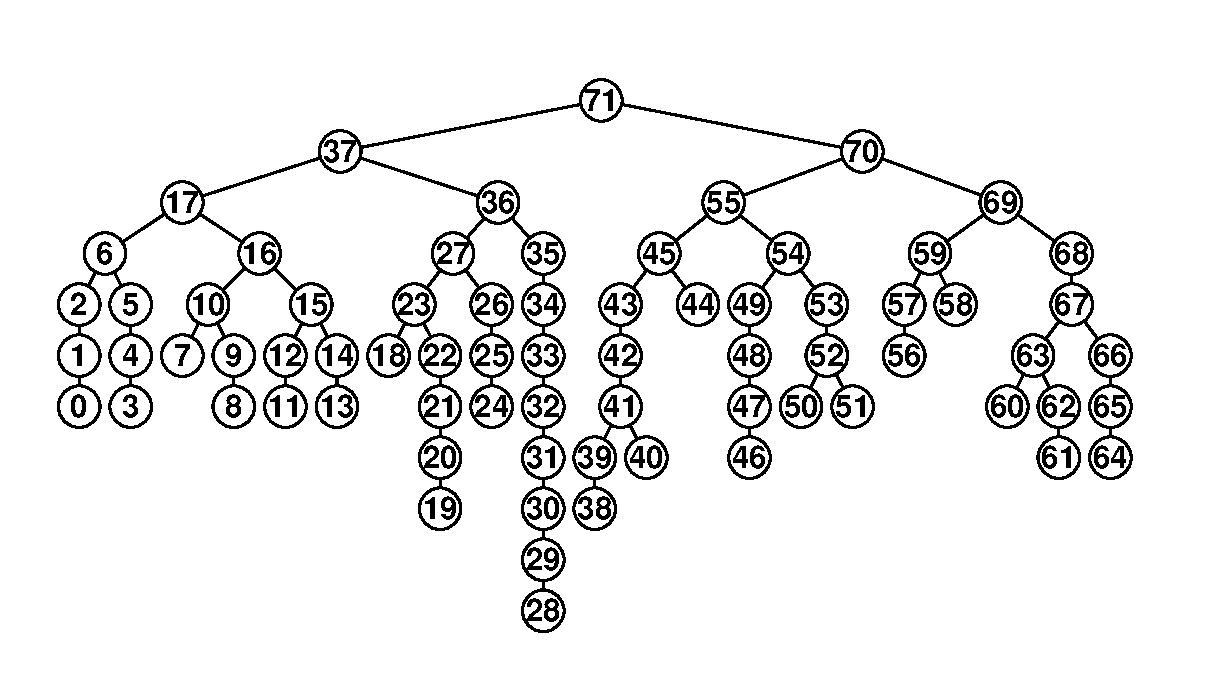
\psfig{file=fstree.eps,width=4.71in,height=2.63in}
}
\end{center}
\end{figure}
\par
\begin{figure}[htbp]
\caption{Block structure of $L$ with the fundamental supernode
partition.}
\label{fig:R2D100-fs-mtx}
\begin{center}
\mbox{
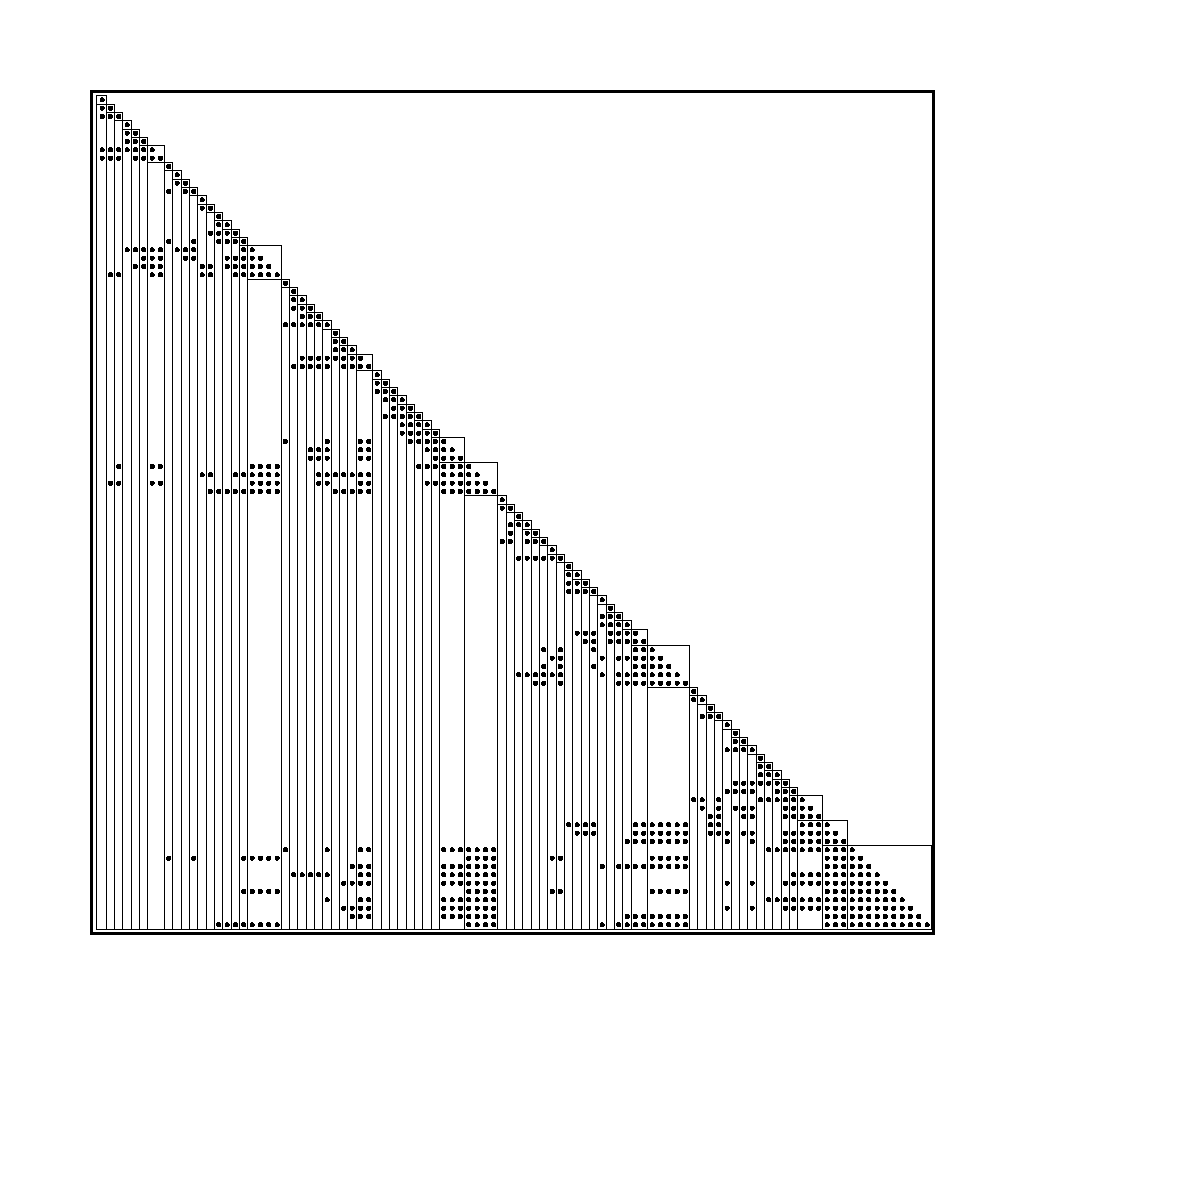
\psfig{file=fsmtx.eps,width=5.0in,height=5.00in}
}
\end{center}
\end{figure}
\par
The code fragment to convert a tree into a fundamental supernode tree is
given below.
\begin{verbatim}
ETree   *fsetree, *vetree ;
int     maxzeros ;
IV      *nzerosIV ;

nzerosIV = IV_new() ;
IV_init(nzerosIV, vetree->nfront, NULL) ;
IV_fill(nzerosIV, 0) ;
maxzeros = 0 ;
fsetree = ETree_mergeFrontsOne(vetree, maxzeros, nzerosIV) ;
\end{verbatim}
The {\tt ETree\_mergeFrontsOne()} method constructs a new {\tt ETree}
object from the {\tt vetree} object.
When a node $J$ has a single child $I$, it looks to see whether merging
$I$ and $J$ together will add more than a given number of zeroes into
the block columns of $I$ and $J$.
(The nonzero rows of the block of $I$ and $J$ together is the union of
the nonzero rows of blocks $I$ and $J$ separately, and all nonzero rows
are stored as dense rows.)
To create a fundamental supernode tree, the number of
zeros allowed into a block column is zero, i.e., the nonzero structure 
of the fundamental supernode tree contains no zeros.
The {\tt nzerosIV} object contains a running count of the number of zero
entries present in the factor storage.
It will be used in later calls to other transformation methods.
\par
\subsection{Amalgamated or relaxed supernode trees}
\label{subsection:am-tree}
\par
A factorization based on the fundamental supernode tree requires
no more operations than one based on the vertex elimination tree.
There are many small supernodes at the lower levels of the tree. 
By {\it amalgamating} small but connected sets of supernodes together 
into larger supernodes we can reduce the overhead of the processing 
all of the small supernodes at the expense of adding
entries to the factors and operations to compute the factorization.
This amalgamation of supernodes generally leads to an overall 
increase in efficiency
\cite{ash89-relaxed},
\cite{duf83-multifrontal}.
We call the result the {\it amalgamated} 
or {\it relaxed} supernode tree.
\par
The top tree in Figure~\ref{fig:am-trees}
shows the vertex elimination tree with the ``front'' number of each
vertex superimposed on the vertex.
The bottom tree is the amalgamated supernode tree.
Figure~\ref{fig:R2D100-am-mtx} shows the block partition superimposed on
the structure of the factor $L$.
\par
\begin{figure}[htbp]
\caption{Top: fundamental supernode tree with the supernodes mapped to
the amalgamated supernode that contains them. 
Bottom: amalgamated supernode tree.}
\label{fig:am-trees}
\begin{center}
\mbox{
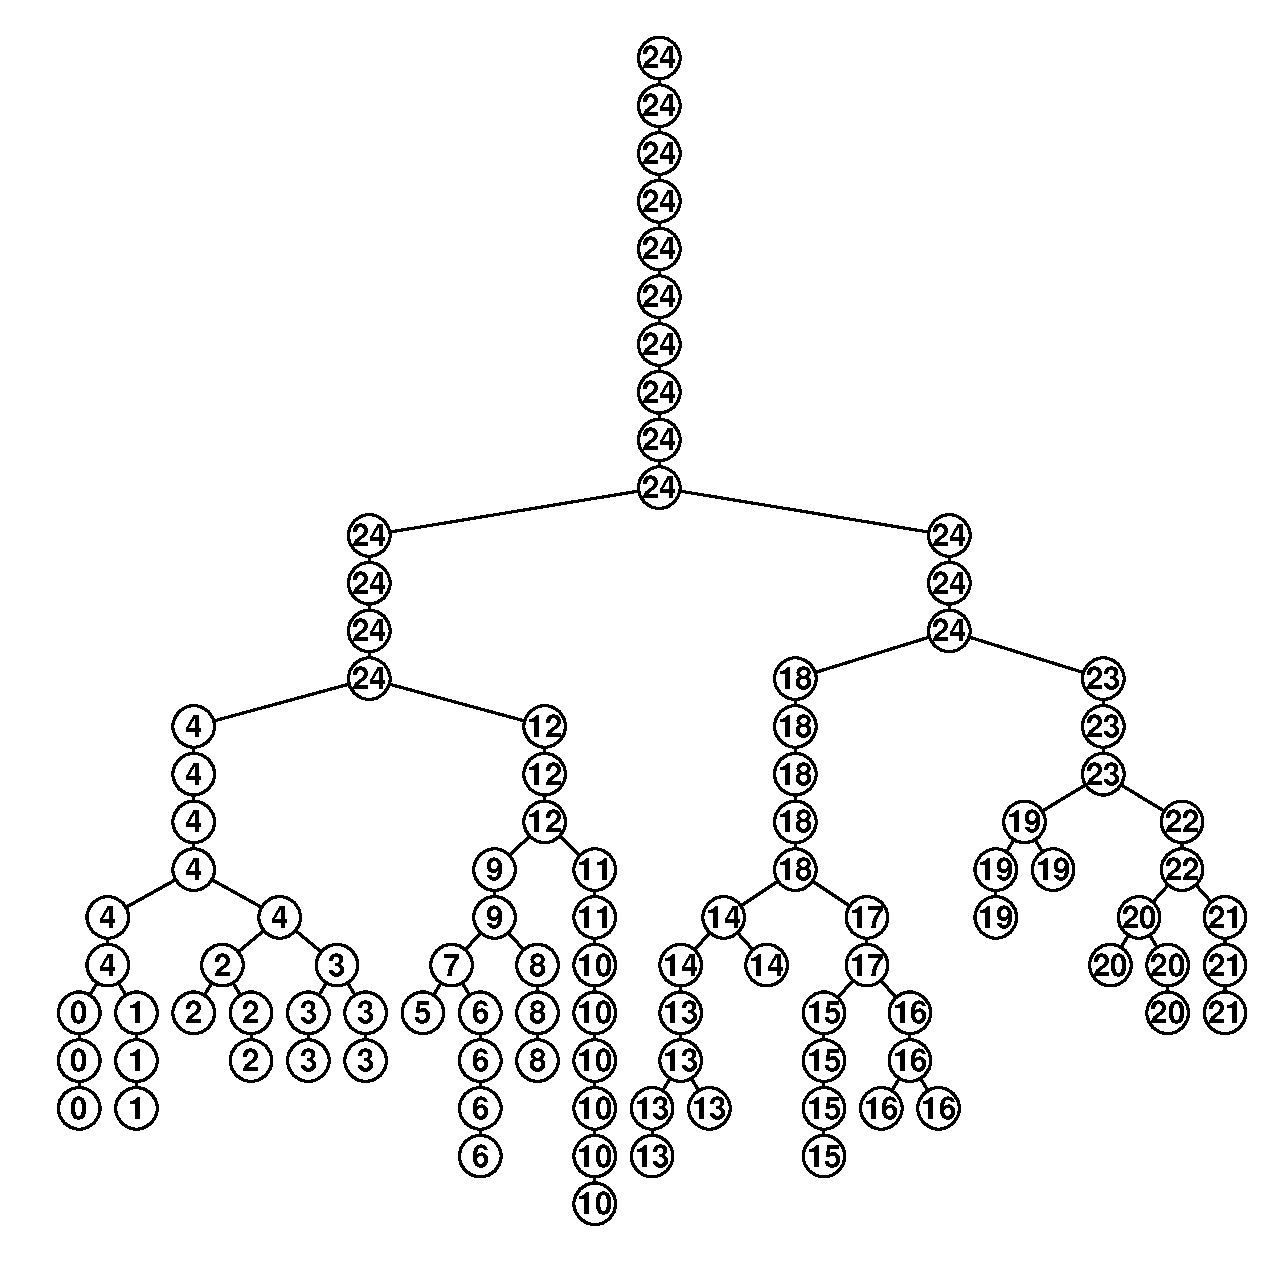
\psfig{file=amvtree.eps,width=5.0in,height=5.00in}
}
\par
\mbox{
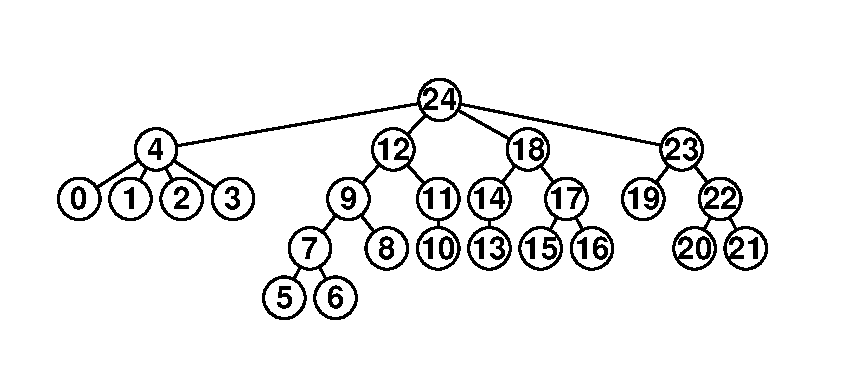
\psfig{file=amtree.eps,width=3.25in,height=1.38in}
}
\end{center}
\end{figure}
\par
\begin{figure}[htbp]
\caption{Block structure of $L$ with the amalgamated supernode
partition.}
\label{fig:R2D100-am-mtx}
\begin{center}
\mbox{
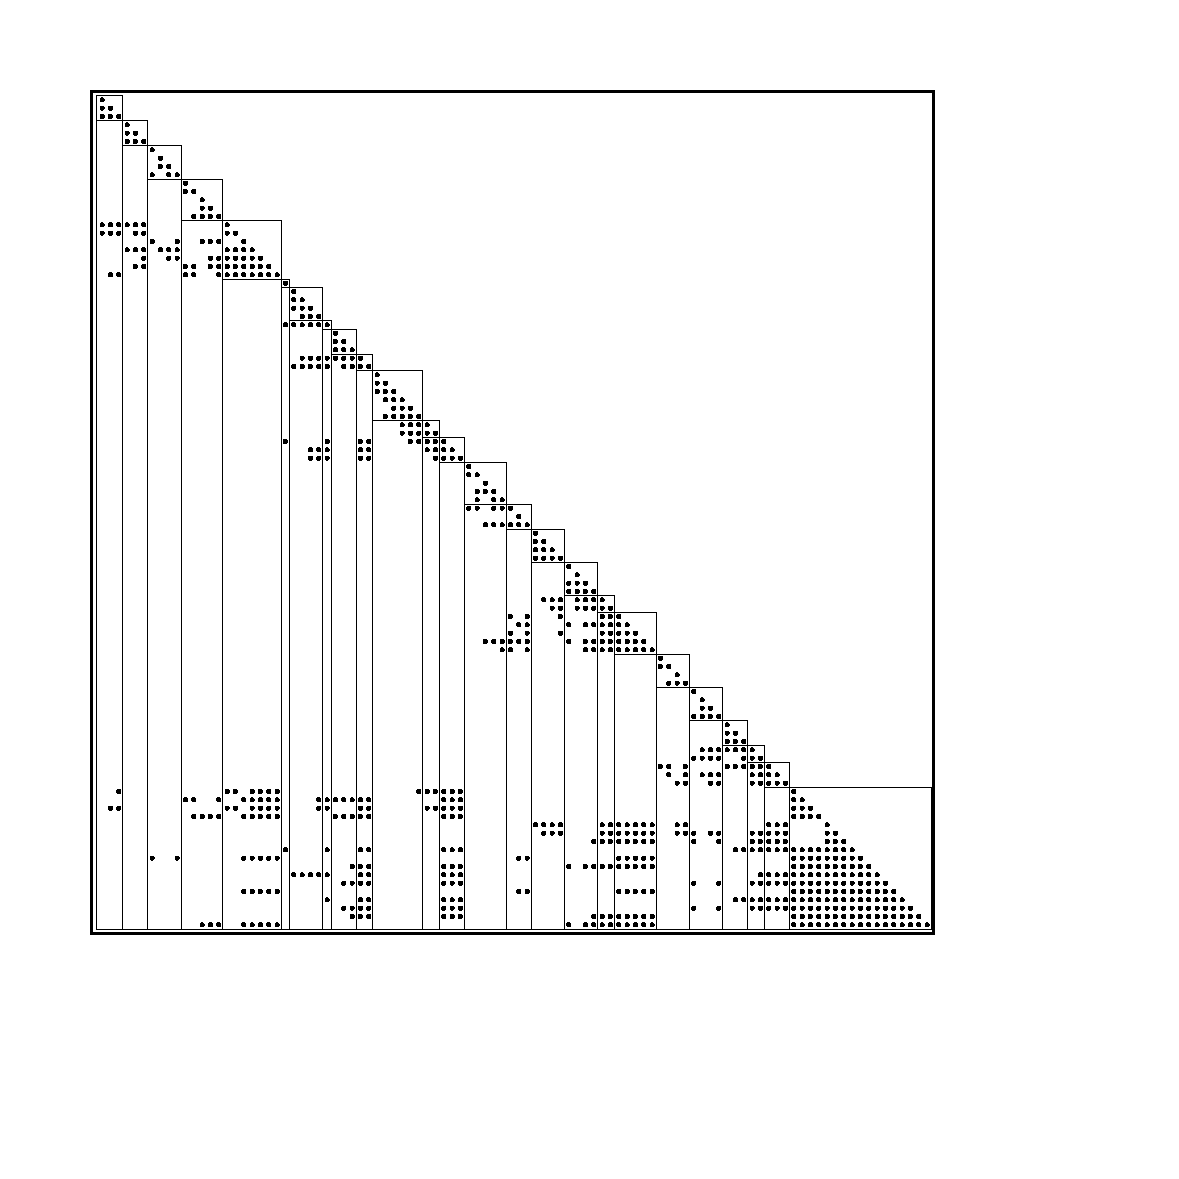
\psfig{file=ammtx.eps,width=5.0in,height=5.00in}
}
\end{center}
\end{figure}
\par
The code fragment to create this amalgamated tree is found below.
\begin{verbatim}
ETree   *ametree ;

maxzeros = 20 ;
ametree = ETree_mergeFrontsAll(fsetree, maxzeros, nzerosIV) ;
\end{verbatim}
This method will merge a node with {\it all} of its children if it will
not result in more than {\tt maxzeros} zeros inside the new block.
On input, {\tt nzerosIV} object keeps count of the number of zeroes 
already in the blocks of {\tt fsetree}, and on return it will
contain the number of zeros in the blocks of {\tt ametree}.
\par
\subsection{Splitting large fronts}
\label{subsection:sp-tree}
\par
There is one final step to constructing the tree that governs the
factorization and solve.
Large matrices will generate large supernodes at the topmost levels
of the tree.
For example, a $k \times k \times k$ grid with a 27 point finite
difference operator, when ordered by nested dissection, has a root
supernode with $k^2$ rows and columns.
The data structure for a top level supernode can be very large,
too large to fit into memory.
In a parallel environment, we follow the convention that each node
in the tree is handled by one process.
Having a very large node at the top levels of the tree will
severely decrease the parallelism available to the computations.
\par
The solution to both problems, large data structures and limited
parallelism, is to split large supernodes into pieces.
We can specify a maximum size for the nodes in the tree, and split
the large supernode into pieces no larger than this maximum size.
This will keep the data structures to a manageable size and increase
the available parallelism.  We call the resulting tree the {\it front}
tree because it represents the final computational unit for the
factorization, the frontal matrix.
\par
The amalgamated supernode tree has been transformed so that except for
the leaf nodes, which are not changed, no node in the tree has more 
than four vertices.
The top tree in Figure~\ref{fig:sp-trees}
shows the vertex elimination tree with the ``front'' number of each
vertex superimposed on the vertex.
The bottom tree is the amalgamated and split supernode tree.
Figure~\ref{fig:sp-mtx} shows the block partition superimposed on
the structure of the factor $L$.
Splitting large nodes into smaller nodes will not increase the
factor storage or operation counts, in fact, as we shall soon see,
it is possible to decrease them slightly when compared to the
amalgamated tree before splitting.
\par
\begin{figure}[htbp]
\caption{Left: tree after the large supernodes have been split.
Right: tree with nodes mapped back to their amalgamated supernode.}
\label{fig:sp-trees}
\begin{center}
\mbox{
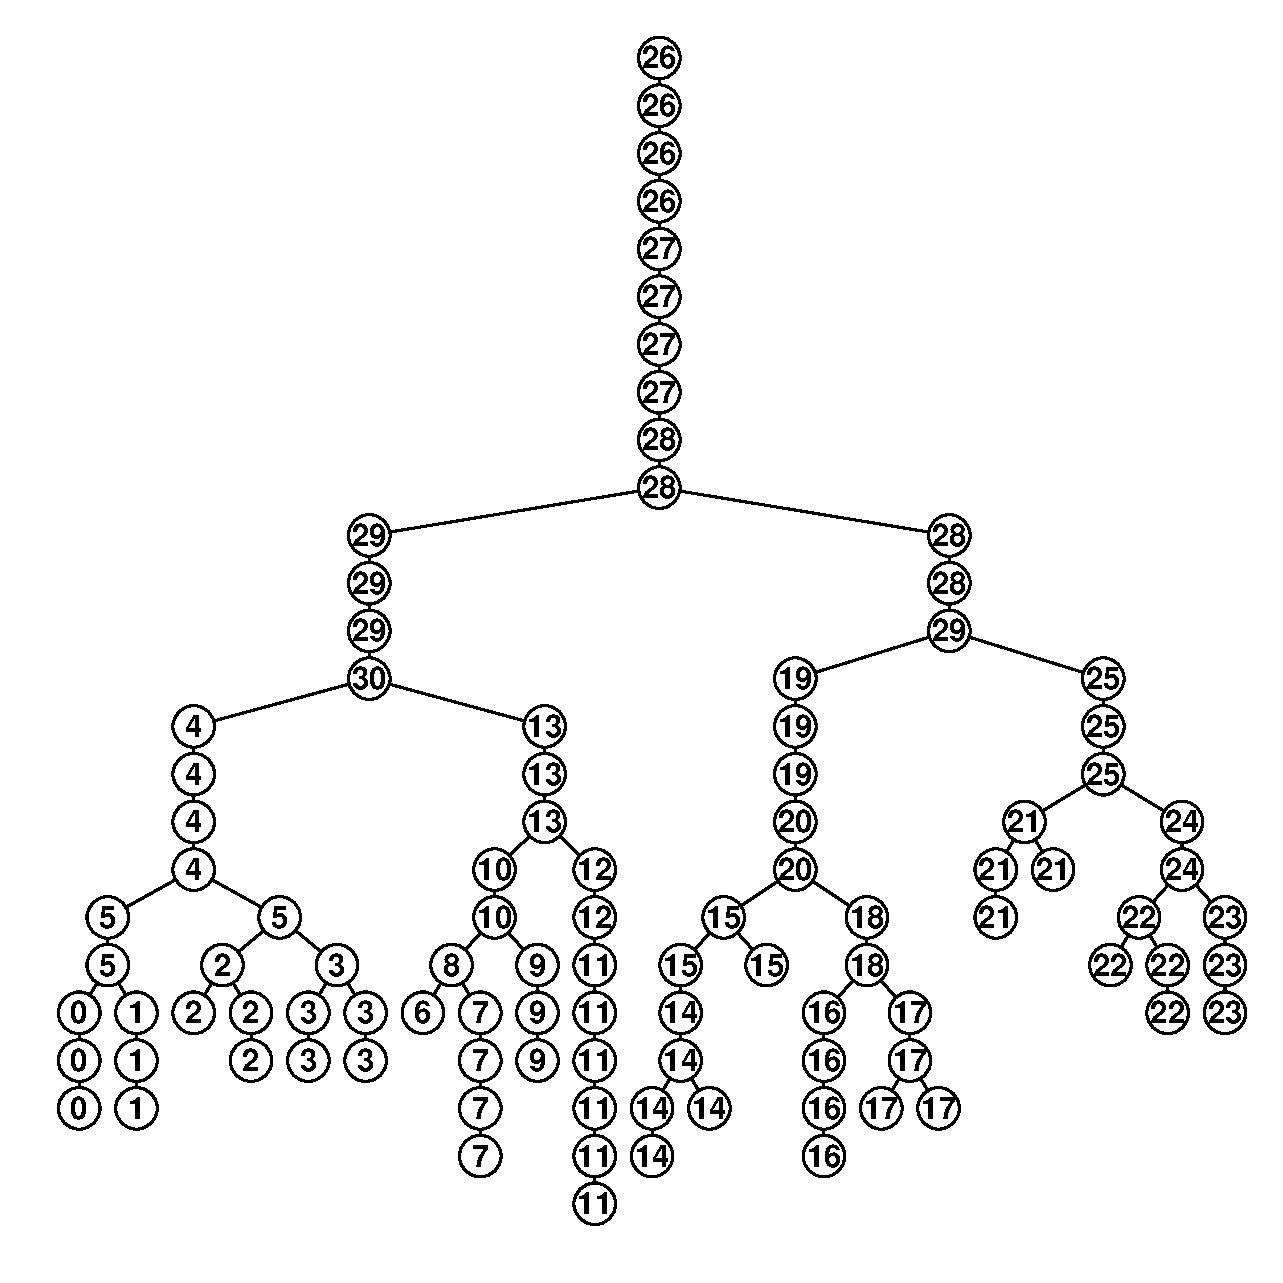
\psfig{file=spvtree.eps,width=5.00in,height=5.000in}
}
\quad
\mbox{
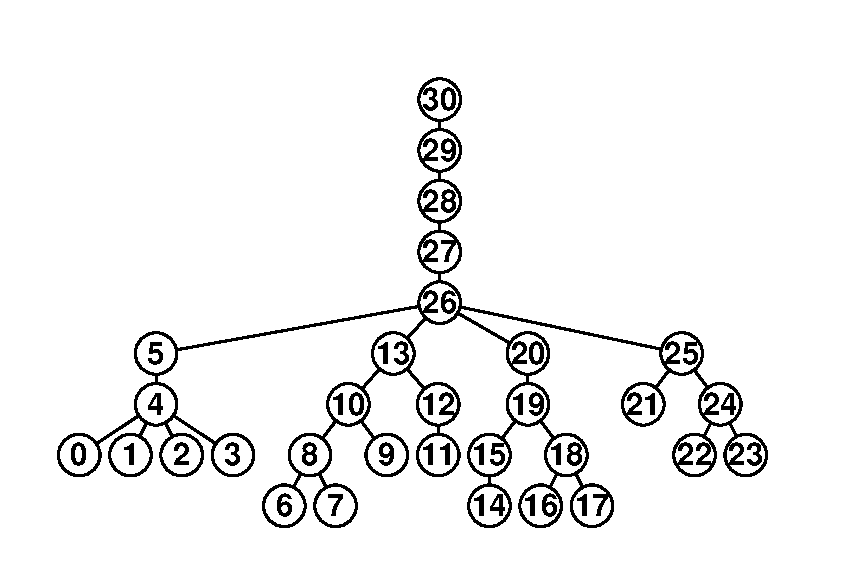
\psfig{file=sptree.eps,width=3.25in,height=2.21in}
}
\end{center}
\end{figure}
\par
\begin{figure}[htbp]
\caption{Block structure of $L$ with the amalgamated and split
         supernode partition.}
\label{fig:sp-mtx}
\begin{center}
\mbox{
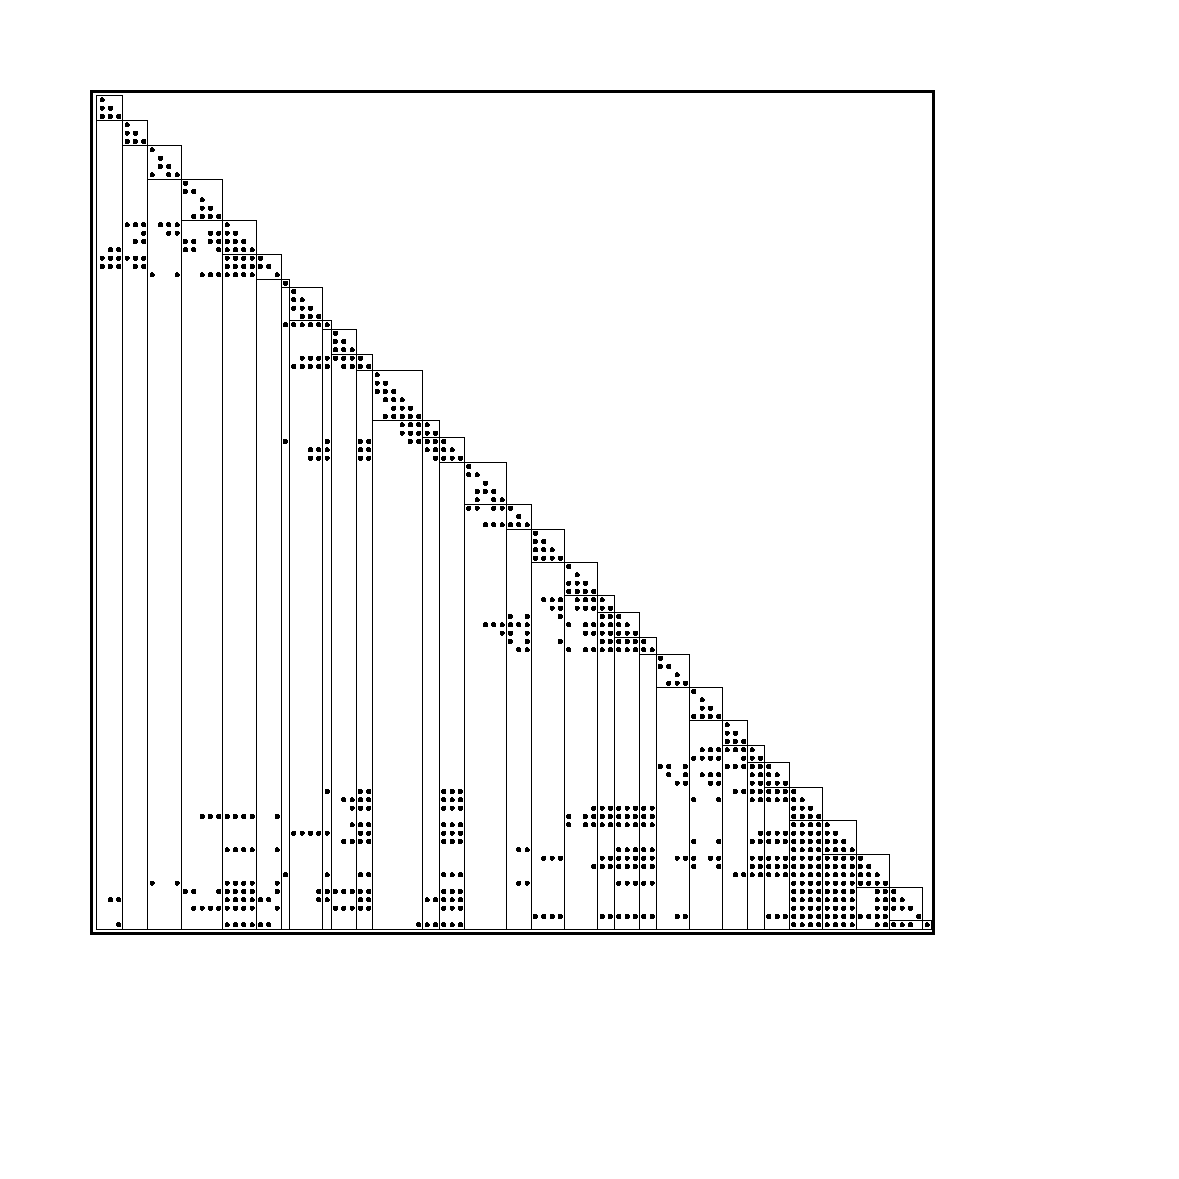
\psfig{file=spmtx.eps,width=5.0in,height=5.00in}
}
\end{center}
\end{figure}
\par
The code fragment to split the large fronts is found below.
\begin{verbatim}
ETree   *spetree ;
int     maxsize, seed ;

maxsize = 4 ;
spetree = ETree_splitFronts(ametree, NULL, maxsize, seed) ;
\end{verbatim}
This method creates and returns an {\tt ETree} object where each front
has {\tt maxsize} or fewer internal rows and columns, except for the
fronts that are leaves in the tree.
Here we imposed the condition that no non-leaf front has more than four
vertices.
The second parameter in the calling sequence is non-{\tt NULL} 
if the graph has nonunit vertex weights.
The last parameter is a seed for a random number generator.
When we identify a front with more than {\tt maxsize} internal rows and
columns, there are many ways to split the front into smaller fronts.
We try to keep the sizes of the fronts roughly equal, but which vertices
to play into which fronts is not specified.
We shuffle the vertices using a random number generator and assign
vertices to smaller fronts in a block manner.
\par
\subsection{Results}
\label{subsection:tree-results}
\par
This front tree is now the defining
structure for the numerical factorization and solve steps.  
The structure of the front tree defines the order of the computations 
that will be carried out in the factorization and the solve.  
The composition of the front tree can have a profound effect on storage
and performance of the factorization and solves.
\par
Our {\tt R2D100} matrix was small enough to illustrate the steps in the
transformation of the front tree, but is not large enough to 
realistically display how the front tree influences the differences 
in storage and speed of the computations.
Now we look at the {\tt R3D13824} matrix.
Table~\ref{table:R3D13824-tree-stats} contains some statistics for a
sequence of front trees.
The original front tree came from our nested dissection ordering.
\par
\begin{table}[htbp]
\label{table:R3D13824-tree-stats}
\caption{R3D13824: front tree transformations}
\begin{center}
\begin{tabular}{l|rrrrr}
& CPU & \# fronts & \# indices & \# entries & \# operations \\ \hline
 original  &        &  6001 & 326858 & 3459359 & 1981403337 \\
 fs tree   & 0.040  &  6000 & 326103 & 3459359 & 1981403337 \\
 merge one & 0.032  &  3477 & 158834 & 3497139 & 2000297117 \\
 merge all & 0.020  &   748 &  95306 & 3690546 & 2021347776 \\
 merge any & 0.012  &   597 &  85366 & 3753241 & 2035158539 \\
 split     & 0.043  &   643 & 115139 & 3753241 & 2035158539 \\
 final     & 0.423  &   643 & 115128 & 3752694 & 2034396840
\end{tabular}
\end{center}
\end{table}
\par
There are 13824 rows and columns in the matrix, and 6001 fronts in the
nested dissection tree.
While there is an average of two rows and columns per front,
most of the fronts are singleton fronts at the lower levels of the tree.
The top level front has 750 internal rows and columns.
\par
\begin{itemize}
\item
In the first step we create an fundamental supernode tree with a call to
{\tt ETree\_mergeFrontsOne()} with {\tt maxzeros = 0}.
We see that the number of fronts decreases by one and the number of
entries does not change.
\item
The second step is also a call to
{\tt ETree\_mergeFrontsOne()}, this time with {\tt maxzeros = 1000}.
Here we merge fronts with only one child with that child,
in other words, only chains of nodes can merge together.
Note how the number of fronts is decreased by almost one half, 
and the number of factor entries and operations increase by 1\%.
\item
The third step is a call to {\tt ETree\_mergeFrontsAll()}
with {\tt maxzeros = 1000}, where we try
to merge a node with all of its children if possible.
The number of fronts decreases again by a factor of five, while the
number of factor entries and operations increases by 7\% and 2\%,
respectively, when compared with the original factor matrices.
\item
The fourth step 
is a call to {\tt ETree\_mergeFrontsAny()}
with {\tt maxzeros = 1000}, where we try
to merge a front with any subset of its children.
The number of fronts decreases further, and the factor entries and
operations increase by 8\% and 3\%, respectively.
\item
In the fifth step 
is a call to {\tt ETree\_splitFronts()}
with {\tt maxsize = 64}, where we try
split the large fronts into smaller fronts.
Note that the number of factor entries and operations do not seem to
increase, while the number of fronts increases by about 8\%.
In reality, a large front that is split into smaller fronts may have a
non-dense block column structure, a one of its smaller fronts may have 
rows in its block column of $L$ that are zero, whereas that same row in
the larger front is nonzero.
\end{itemize}
Merging fronts and splitting fronts can have a large effect on the
computational performance of a factor and solve.
Table~\ref{table:R3D13824-comp-stats} contains some results for
solving linear systems of equations for the {\tt R3D13824} matrix
using the five different front trees.
\par
\begin{table}[htbp]
\label{table:R3D13824-comp-stats}
\caption{R3D13824: 
         factor and solve timings for five different front trees.}
\begin{center}
\begin{tabular}{l|ccccccc}
& & \multicolumn{2}{c}{factor} & & \multicolumn{2}{c}{solve} & total \\
& init & CPU & mflops & postprocess & CPU & mflops & CPU \\ \hline
 original  & 4.0 & 131.7 & 15.0 & 5.0 & 7.3 & ~7.6 & 148.0 \\
 fs tree   & 3.3 & 130.4 & 15.2 & 5.4 & 7.8 & ~7.1 & 146.9 \\
 merge one & 3.1 & 119.9 & 16.7 & 2.7 & 4.6 & 12.1 & 130.3 \\
 merge all & 3.0 & 120.7 & 16.7 & 1.4 & 3.6 & 16.2 & 128.7 \\
 merge any & 3.0 & 121.6 & 16.7 & 1.4 & 3.5 & 16.9 & 129.5 \\
 split     & 3.0 & ~84.9 & 24.0 & 1.9 & 3.5 & 17.1 & ~93.3 
\end{tabular}
\end{center}
\end{table}
\par
The first thing to notice is that factorization performance improves
slightly as small fronts are merged together.
The large improvement comes when the fronts are split.
The explanation of this behavior is that all {\it inter-front}
computation is done using BLAS3 kernels for the operation
$Y := Y - L * D * U$, where $L$ and $U$ are dense matrices,
$D$ is diagonal or block diagonal with $1 \times 1$ and $2 \times 2$
pivots, and $Y$ is dense.
The {\it intra-front} computations, done entirely within the block
columns of $L$ and block rows of $U$, are done using BLAS1 kernels.
This is necessary when pivoting for stability.
Had we chosen to write BLAS3 kernels for the intra-front
computations when pivoting is not enabled, the factorization timings for
the first five front trees would have been higher.
But splitting fronts into smaller fronts is necessary for parallel
computations, so it made sense to make it the recommended route for
serial computations as well.
There would be very little difference in speed had the intra-front
computations been done with BLAS3 kernels compared with using the 
final front tree, for the intra-front computations are a small fraction
of the total number of operations.
\par
The solve time improves dramatically when small fronts are merged
together into larger fronts.
Our solves are submatrix algorithms, where the fundamental kernel is an
operation 
$Y_J := B_J - L_{J,I} X_I$
and
$X_J := Y_J - U_{I,J} Y_J$,
and is designed to be a BLAS2 kernel (when $X$ and $Y$ have a single
column) or BLAS3 kernel (when $X$ and $Y$ are matrices).
When fronts are small, particularly with one internal row and column,
the submatrices that take part are very small.
The overhead for the computations takes far more time than the
computations themselves.
\par
This multistep process of merging, merging again, etc, and finally 
splitting the front trees is tedious.
There are simple methods that do the process in one step.
\begin{verbatim}
ETree   *etree, *etree2, *etree3 ;
int     maxfrontsize, maxzeros, seed ;

etree2 = ETree_transform(etree, NULL, maxzeros, maxfrontsize, seed) ;
etree3 = ETree_transform2(etree, NULL, maxzeros, maxfrontsize, seed) ;
\end{verbatim}
Inside The {\tt ETree\_transform()} method 
is a sequence of four transformations:
\begin{itemize}
\item
Merge small fronts into larger fronts
using the {\tt ETree\_mergeFrontsOne()} method.
\item
Then merge small fronts into larger fronts
using the {\tt ETree\_mergeFrontsAll()} method.
\item
Then merge small fronts into larger fronts
using the {\tt ETree\_mergeFrontsAny()} method.
\item
Then merge a large front into a chain of smaller fronts
using the {\tt ETree\_splitFronts()} method.
\end{itemize}
The {\tt ETree\_transform2()} method differs from the 
{\tt ETree\_transform()} method in that it omits the
setp with {\tt ETree\_mergeFrontsAny()}.
Either method will be suitable in most cases.
\par
However, there are some times one method is to be preferred over
the other.
If we look again at the vertex elimination tree
in Figure~\ref{fig:R2D100-tree-vtx}, we see the top level separator
with nodes $\{90,\cdots,99\}$, and the two second level separators
with nodes $\{45,\cdots,47\}$ and $\{87,\cdots,89\}$.
If one looks at their block columns in Figure~\ref{fig:R2D100-fs-mtx}
we see that either of the two second level separators could be merged
with the top level separator without introducing any zero entries
into the factor.
Using the {\tt ETree\_mergeFrontsAny()} method could merge the top
level separator with one of its two children, and produce an
imbalanced tree, not as well suited for parallel computation had
the two separators not been merged.
\par
In a parallel environment, it is much more efficient to not merge 
the top level separator with either of its second level separators.
The transformation methods in {\bf SPOOLES 1.0} created front trees that
were not as efficient for parallel processing, precisely because of
the use of the ``merge-with-any'' step.
This led us to write three separate merging methods to replace the
single method from the 1.0 release, and thus give us the ability to
avoid the trees unsuitable for parallel computation.
\par
The values of {\tt maxzeros} and {\tt maxsize} will have a fair
amount of influence on the efficiency of the factor and solves.
This is illustrated in Table~\ref{table:R3D13824-maxzero-maxsize}
for the {\tt R3D13824} matrix and a number of different combinations 
of {\tt maxzeros} and {\tt maxsize}.
\par
\begin{table}[htbp]
\label{table:R3D13824-maxzero-maxsize}
\caption{R3D13824: the influence of {\tt maxzeros} and {\tt maxsize}.}
\begin{center}
\begin{tabular}{cc|ccccccc}
& & & \multicolumn{2}{c}{factor} & & \multicolumn{2}{c}{solve} & total\\
{\tt maxzeros} & {\tt maxsize} 
   & init & CPU & mflops & postprocess & CPU & mflops & CPU \\ \hline
$~~~~~0$ & $\infty$ & 3.3 & 129.8 & 15.3 & 5.3 & 7.8 & ~7.1 & 146.2 \\
$~~~~10$ & $\infty$ & 3.5 & 129.2 & 15.3 & 3.3 & 5.3 & 10.5 & 141.3 \\
$~~~100$ & $\infty$ & 3.0 & 119.3 & 16.7 & 2.0 & 3.9 & 14.4 & 128.2 \\
$~~1000$ & $\infty$ & 3.0 & 121.8 & 16.7 & 1.4 & 3.5 & 17.0 & 129.7 \\
$~10000$ & $\infty$ & 3.5 & 138.1 & 16.8 & 1.5 & 4.0 & 17.8 & 147.1 \\
$~~1000$ &    32    & 3.3 & ~89.8 & 22.7 & 2.6 & 4.1 & 14.7 & ~99.8 \\
$~~1000$ &    48    & 3.1 & ~85.8 & 23.7 & 2.1 & 3.6 & 16.5 & ~94.6 \\
$~~1000$ &    64    & 3.1 & ~85.2 & 23.9 & 1.9 & 3.5 & 17.1 & ~93.7 \\
$~~1000$ &    80    & 3.0 & ~85.9 & 23.7 & 1.8 & 3.4 & 17.4 & ~94.1 \\
$~~1000$ &    96    & 3.0 & ~86.1 & 23.6 & 1.8 & 3.4 & 17.6 & ~94.3 \\
$~~~~~0$ &    32    & 3.3 & 100.3 & 19.8 & 6.6 & 7.9 & ~7.0 & 118.1 \\
$~~~~~0$ &    48    & 3.2 & ~97.0 & 20.4 & 6.1 & 7.6 & ~7.3 & 113.9 \\
$~~~~~0$ &    64    & 3.2 & ~95.8 & 20.7 & 5.4 & 6.9 & ~8.0 & 111.3 \\
$~~~~~0$ &    80    & 3.2 & ~96.7 & 20.5 & 5.5 & 7.1 & ~7.8 & 112.5 \\
$~~~~~0$ &    96    & 3.2 & ~97.2 & 20.4 & 5.2 & 6.7 & ~8.3 & 112.3 
\end{tabular}
\end{center}
\end{table}
\par
\par
As the matrix size grows, the number of zero entries we can allow
into a front can also grow.
We recommend using {\tt maxzeros} somewhere between 
{\tt 0.01*neqns} and {\tt 0.1*neqns}.
The exact value isn't crucial, what is important is to have the
smaller subtrees at the lower levels of the tree merged together.
The {\tt maxsize} parameter specifies the ``panel'' size of the
large fronts, and so influences the granularity of the BLAS3
computations in the factorization and solve.
If {\tt maxsize} is too large, then too much of the computations
in the factorization is done inside a front, which uses a slow
kernel.
If {\tt maxsize} is too small, then the fronts are too small to get
much computational efficiency.
We recommend using a value between {\tt 32} and {\tt 96}.
Luckily, the factor and solve times are fairly flat within this
range.
A value of {\tt 64} is what we customarily use.
